\section{Testing and Observations}
\label{section:testing_and_observations}
\subsection{Keypad Debouncing}
Our first component that required testing was the keypad, which unfortunately did not have a formal datasheet available. An important required step for us to figure out which output pin was set by the buttons on the keypad. Our approach to debugging this was to connect what was presumed to be the column pins to the digit pins of the display, and then to press the buttons and observe which segment would light up. Once the keypad pins were mapped and each button was assigned a combination of COL and ROW pins, our focus shifted towards debouncing the digit presses. This was achieved using a deboucing interval of 200ms, in combination with a minimum update count, which is described in Section \ref{section:implementation}. During testing, we observed that this debouncing mechanism worked without problems. %Furthermore, to enter consecutive numbers the user would need to press a second time with a 200ms pause between presses to let the controller know that the button had been released character is pressed and a consecutive repeating character is a new character and not a continuation of the initial digit press.

\subsection{ADC Thread}
We initially implemented an additional thread for our ADC that would wake up as soon as the \verb|DMA_buffer_full()| callback was executed by setting a flag. This through testing however showed that the ADC thread would end up blocking the other threads from executing and eventually block our whole program. Figure ? bellow shows our program output and shows the display and keypad threads getting called until only the ADC thread output is shown.



\begin{figure}[h]
\centering
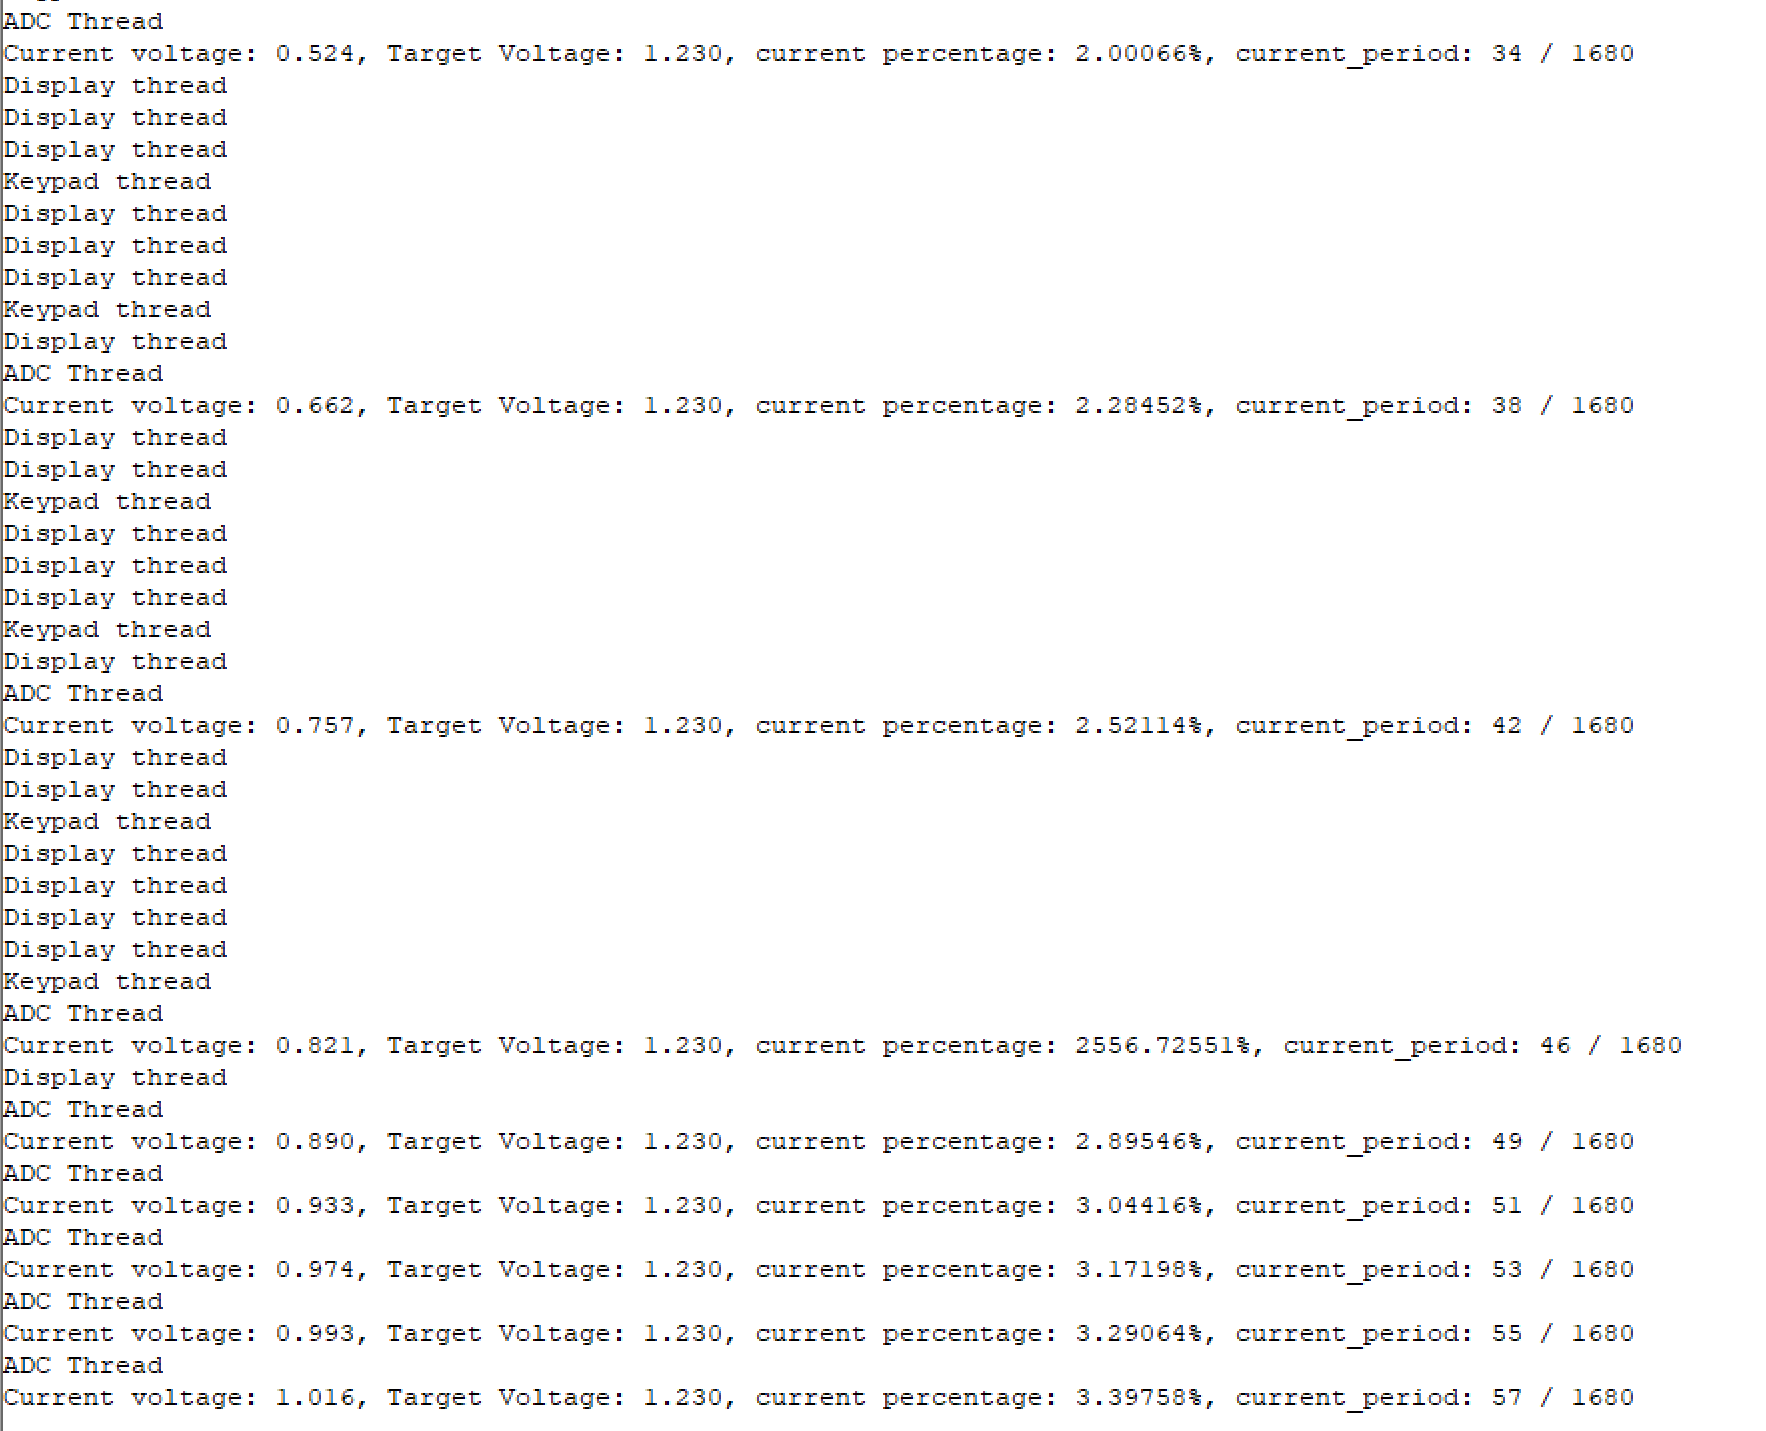
\includegraphics[scale=0.5]{images/weird_behaviour.png}
\caption{
\label{fig:weird_behaviour}
An example of the very weird behaviour observed when using an ADC thread. The ADC, Keypad and Display threads are coexisting peacefully, up until the point at which the ADC thread decides it will keep the CPU all for itself.
}
\end{figure}





To overcome this blocking thread we decided to just keep our ADC DMA processing in a service routine called after every full buffer callback instead of relying on raising the flag to wake up the ADC thread. With this implementation the keypad and display threads would work properly without the blocking that previously occurred.

\subsection{PWM Controller Testing}
The next component to test was our PWM wave generated by timer 3. In order to make sure our PWM pulse had the correct shape, we connected the oscilloscope to the positive terminal of the diode and plotted the resulting wave form, showed in Figure \ref{fig:PWM_duty_cycle}. 

\begin{figure}[h]
\centering
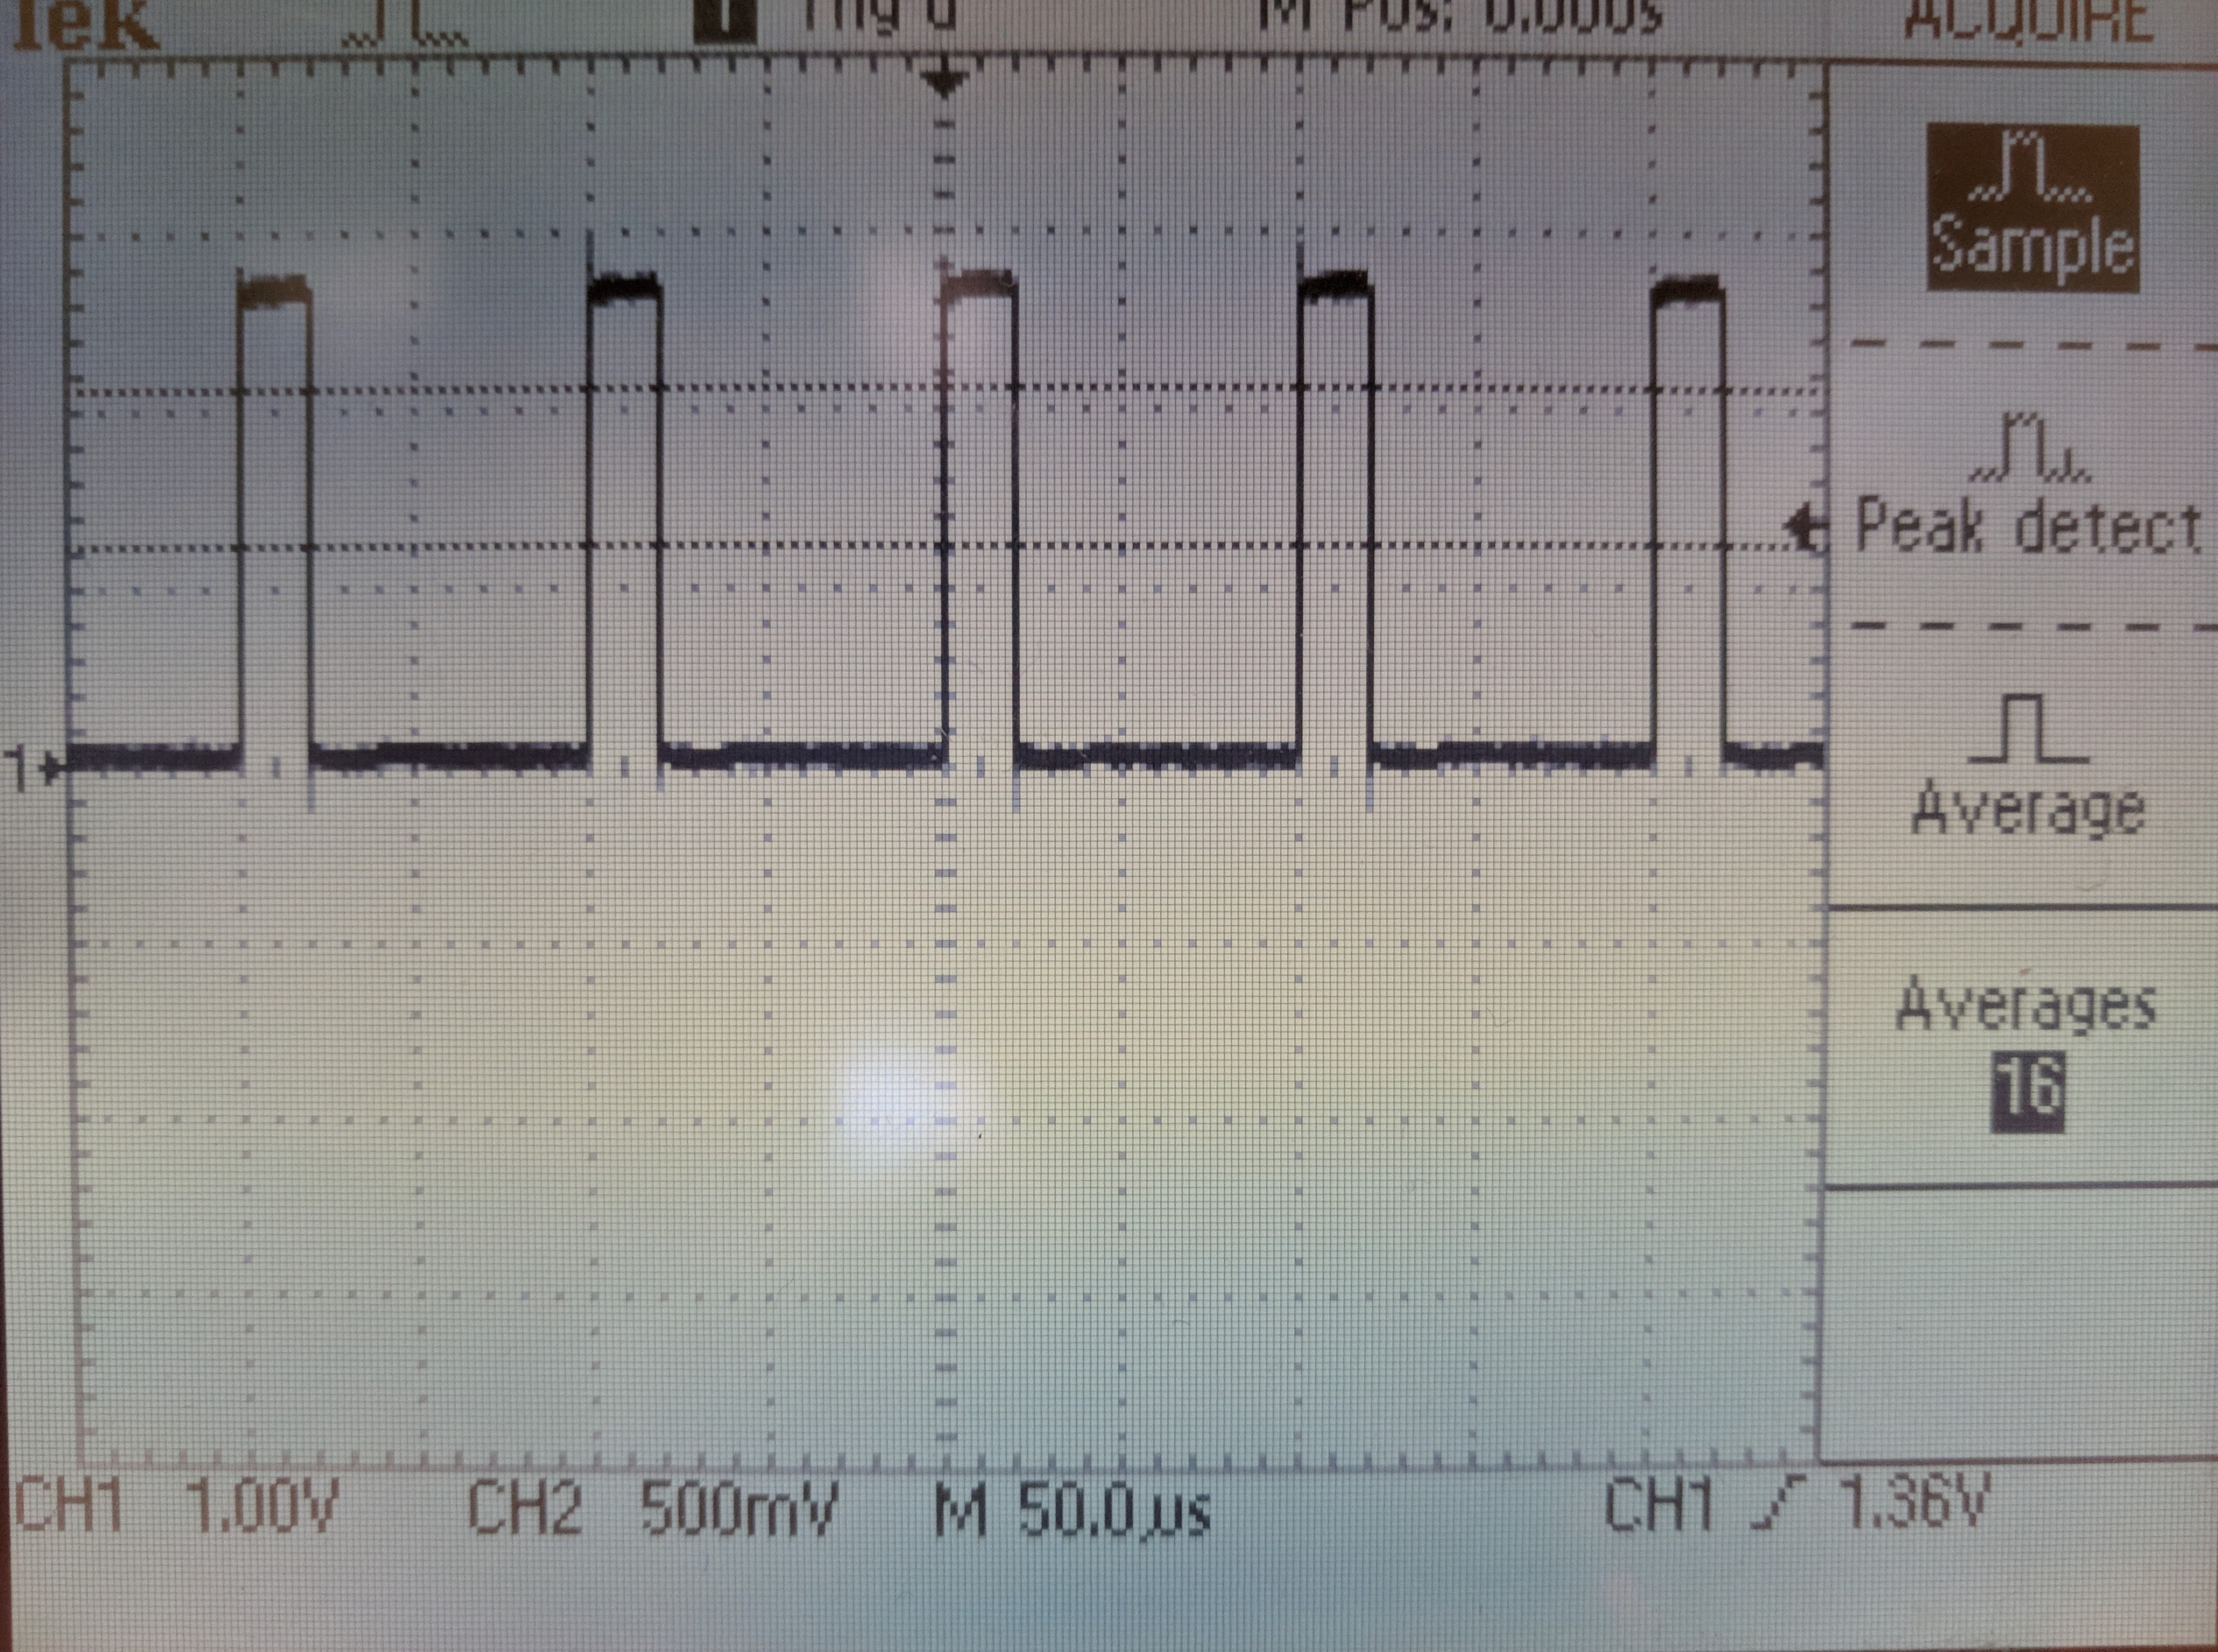
\includegraphics[scale=0.1]{images/pwm_duty_cycle.jpg}
\caption{\label{fig:PWM_duty_cycle} Sample of the PWM signal. The duty cycle appears to be around 25\%.}
\end{figure}


Our first controller, whose code was previously shown in Figure \ref{fig:pwm_controller_1_logic}, was modified from the idea first introduced in Section \ref{section:theory_and_hypothesis} (Theory and Hypothesis). It can be seen working in \ref{fig:pwm_controller_1}. Because this controller adjusts the duty cycle proportionally to the difference between the measured and target RMS values, it fails to reach the target RMS value near the end of the adjustments, partly due to the fact that the difference grows smaller, hence the change in duty cycle also becomes smaller.

\begin{figure}[h]
\includegraphics[scale=0.08]{images/pwm_controller_1.jpg}
\caption{\label{fig:pwm_controller_1} Sample of the first PWM controller in action. As can be observed, the controller never reaches the target value of 2.22V (indicated by cursor 2), despite the sample being $8 * 500ms = 4s$ long.}
\end{figure} \pagebreak



In contrasts to the first implemented controller, our second one uses a Binary Search approach that tends to overshoot and re-correct as seen in Figure \ref{fig:pwm_controller_2}. Although this controller is much faster than our first one, it does overshoot,  which may not be ideal depending on the direct implementation this controller may be used in. For instance, if this PWM signal served to power a motor, the motor might jerk before reaching the desired speed, which is very undesirable. For the purposes of this project, this behaviour is tolerable, as it does not violate any requirement.

\begin{figure}[h]
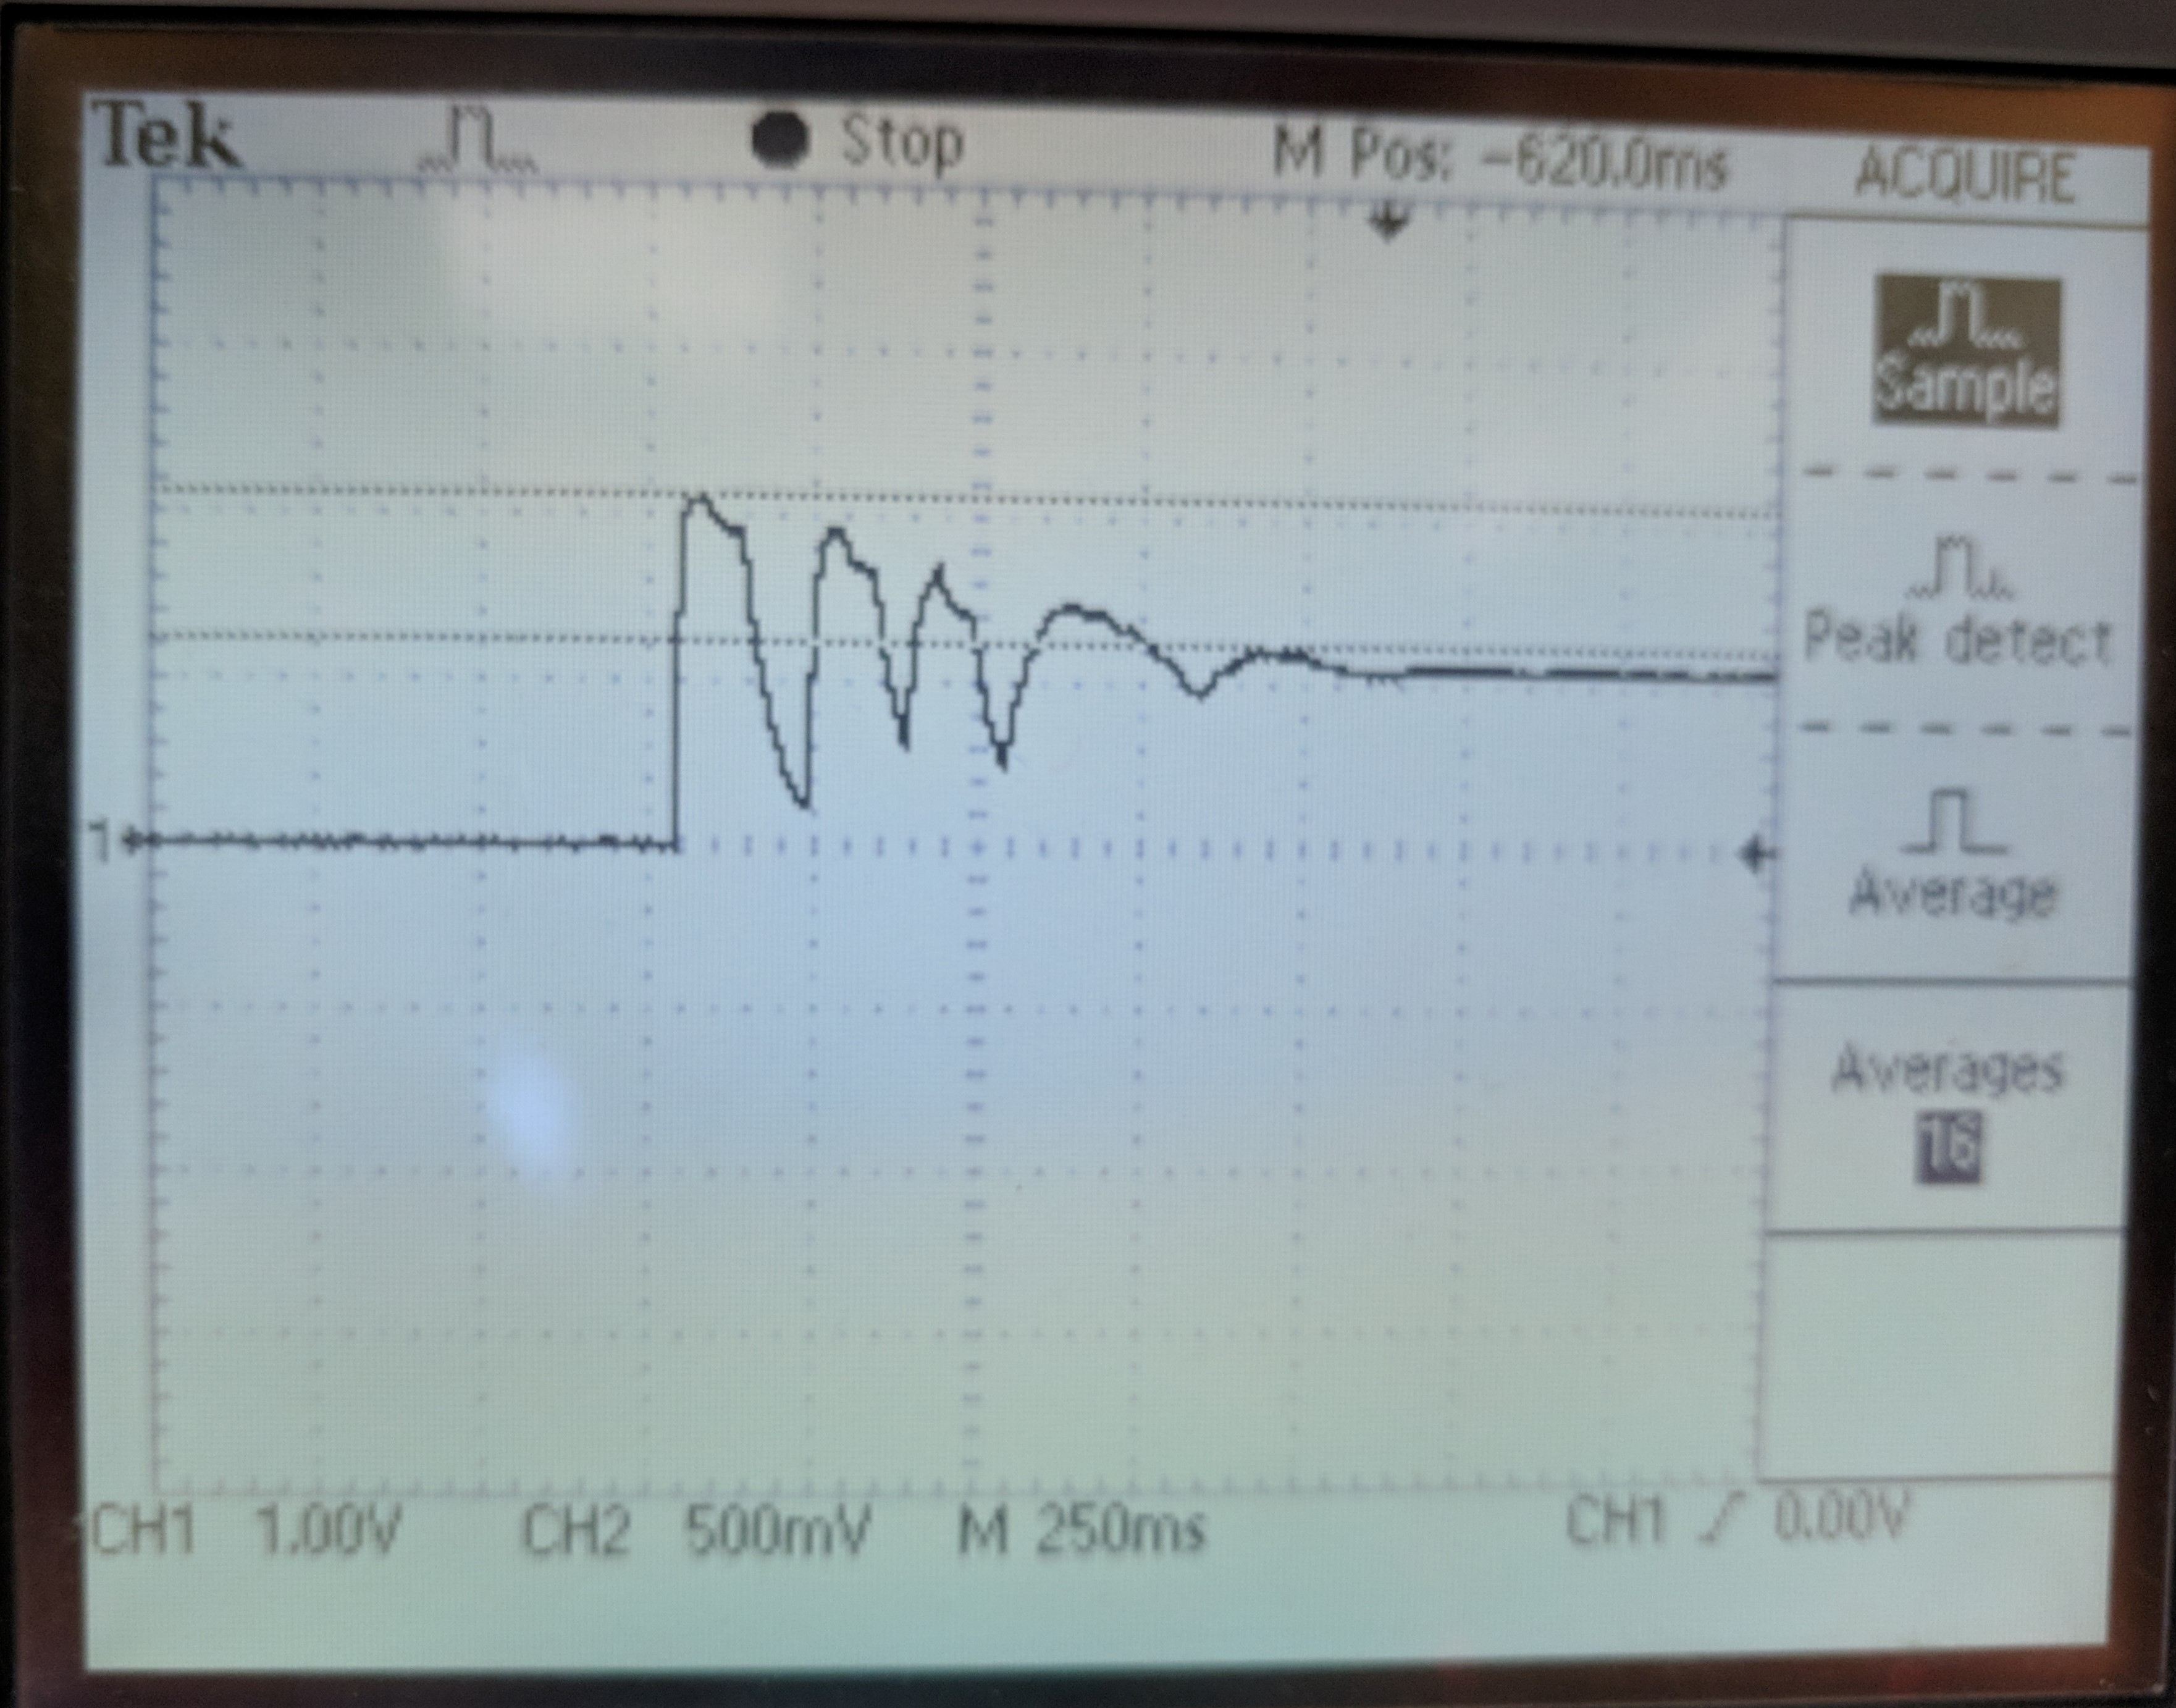
\includegraphics[scale=0.12]{images/pwm_controller_2.jpg}
\caption{\label{fig:pwm_controller_2} Sample of the second PWM controller in action. This controller manages to settle at the desired voltage in about $5 * 250ms = 1.25s$, a very significant improvement upon the first controller.}
\end{figure}

\subsection{Keypad Thread Improvement}



The Keypad thread could be improved in terms of power consumption. In its current state, the keypad thread is using a "polling" mechanism, repeatedly checking each column's GPIO pin to detect if any of them becomes high. Instead, a simple configuration could be devised where all three column pins are each connected to another GPIO pin using diodes. Then, an external interrupt could be used on this pin to wake up the Keypad thread whenever either line becomes high. The keypad thread could then begin polling, counting the time the key has been pressed, up until it is detected that the key has been released. Such a circuit can be seen in Figure \ref{fig:possible_keypad_improvement}. 
\begin{figure}[h]
\begin{circuitikz} \draw

(0,0) to[closing switch, o-, l=COL0] (3,0)
(0,1) to[closing switch, o-, l=COL1] (3,1)
(0,2) to[closing switch, o-, l=COL2] (3,2)
(0,3) to[closing switch, o-, l=COL3] (3,3)
(3,0) to[empty diode, o-] (6,0)
(3,1) to[empty diode, o-] (6,1)
(3,2) to[empty diode, o-] (6,2)
(3,3) to[empty diode, o-] (6,3)
(6,-1) node [below right, rotate=90] {KeyPressed} --  (6, 3)

%(0,0) to[battery] (0,4)
%      to[ammeter] (4,4) 
%      to[C] (4,0) -- (3.5,0)
%      to[lamp, *-*] (0.5,0) -- (0,0)
%(0.5,0) -- (0.5,-2)
%      to[voltmeter] (3.5,-2) -- (3.5,0)
;
\end{circuitikz}
\caption{\label{fig:possible_keypad_improvement} A simple circuit layout which might be more power efficient.}
\end{figure}


The final board arrangement is shown in Figure \ref{fig:board}.
\begin{figure}
\centering
\includegraphics[scale=0.1]{images/circuit.jpg}
\caption{\label{fig:board}The final board setup.}
\end{figure}
